\section{Contexte} % on peut changer "Contexte" pour aurte chose

% Bravo et Félicitations ...

\subsection{Tournoi bicentennal\protect\footnote{périodicité de 200 ans} des Pandas} %  Concours bicentennal de parentage ?

% Côté RP du concours

Comme vous le savez très certainement, la Chine est un grand pays\footnote{9,597 millions km²} regorgeant de traditions vieilles comme le monde\footnote{Nous considèrerons l'arrivée des Ailuropoda melanoleuca (Panda) comme la génèse de ce bas-monde}. L'une d'entre elles est pratiquée, encore à ce jour, par les Pandas Géants et les Pandas Roux. En effet, des observations récentes nous montrent qu'ils pratiquent un rituel, lors duquel la meilleure race de panda est reconnue pour les deux siècles à venir. Par souci d'équité et de justice, le jury n'est pas composé de pandas.
% parler plus du jury ? :thinking:

\subsection{Le championnat}
Le but du championnat est de trouver quelle race compte le meilleur couple de parents\footnote{On remarquera un grand nombre de pédiatres au sein des deux communautés pandesques}. Des bébés pandas seront disposés sur la rivière, dans le grand danger des torrents. Le but des parents est d'aller récupérer tous leurs petits. Le premier couple à avoir récupéré tous les pandas a gagné le match !\footnote{Vous jouerez en effet les deux parents, et non pas un seul panda}

\subsection{Champ de bataille}
Le champ de bataille sera cette année la rivière de \textit{Hulun}, au Nord-Ouest du pays oriental, hôte de ce championnat depuis toujours : la Chine. La rivière, à l'apparence rectangulaire est en fait composée d'hexagones, à travers lesquels des pandas de toutes sortes\footnote{Vous et vos adversaires} devront se mouvoir.

\newpage

\subsubsection{Eau}
L'eau est surprenamment l'élément le plus présent dans la rivière. Il est le premier obstacle. Les pandas ne peuvent pas aller sur l'eau. Ils doivent marcher sur les ponts. Les bébés pandas se trouvent uniquement sur des cases d'eau.

\begin{center}
    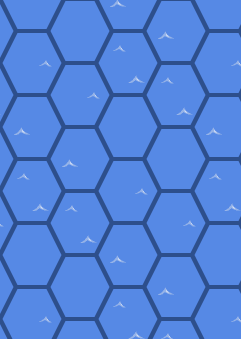
\includegraphics[width=3cm]{water_example.png}
\end{center}

\subsubsection{Ponts}
Les ponts sont le seul moyen de déplacement des pandas. Les ponts sont constitués de deux cases distinctes : une case "+" et une case "-" (en bas à droite des cases de pont). Ces deux cases sont toujours adjacentes\footnote{Sinon, ça ne fait pas un pont.} et reliées par une barre blanche dans l'affichage du match. Chaque case de pont a également une hauteur ou valeur : les nombres en blanc en haut des cases.

\begin{center}
    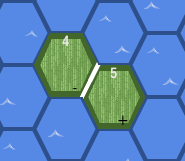
\includegraphics[width=5cm]{bridge_example.png}
\end{center}

Un panda peut se déplacer sur un même pont (à travers le trait blanc) sans contrainte. Pour passer d'un pont à l'autre, il faut que la hauteur du pont duquel le panda part soit la même que celle du pont sur lequel le panda veut aller. C'est le même fonctionnement que les dominos.

\begin{center}
    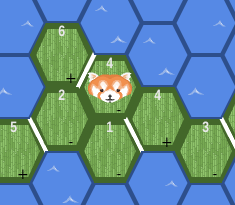
\includegraphics[width=6cm]{lots_of_bridges.png}
\end{center}

Lorsqu'un panda quitte une case d'un pont, la hauteur du pont change. Si c'était une case "+", la hauteur du pont augmente (plus 1 modulo 6). Si la case quittée était une case "-", la hauteur du pont diminue (moins 1 modulo 6). Les valeurs des cases de ponts sont donc toujours incluses entre 1 et 6.

\begin{center}
\begin{tabular}{c c}
     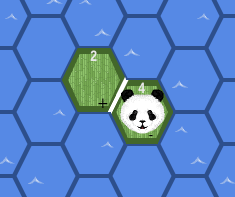
\includegraphics[height=5cm]{bridge_step_1.png} & 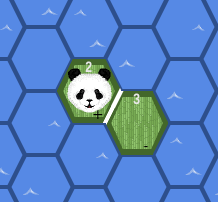
\includegraphics[height=5cm]{bridge_step_2.png} \\
\end{tabular}
\end{center}

\noindent Une fois quelques ponts construits, on peut obtenir ce genre de configuration :

\begin{center}
\begin{figure}[h]
    \centering
    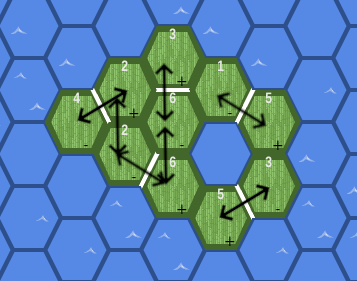
\includegraphics[width=6cm]{beaucoup_de_ponts_avec_fleches.png}
    \caption{Les flèches montrent les déplacements possibles}
\end{figure}
\end{center}

\subsubsection{Rochers}
Les rochers sont les obstacles naturels de la rivière. Rien ne peut traverser ni modifier une case de rocher.

\begin{center}
    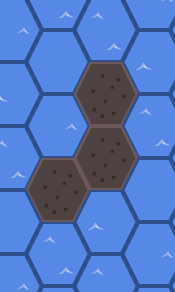
\includegraphics[width=4cm]{a_few_rocks.png}
\end{center}


\subsubsection{Pandas}
Les pandas sont ceux dont vous contrôlez le mouvement. Ils font toutes les actions sur la rivière. Ils peuvent poser des ponts, se déplacer et ramasser les bébés (cette dernière action est automatique). Il y les pandas géants (en noir et blanc), et les pandas roux (en blond vénitien). Ils sont toujours sur un pont.

\begin{center}
    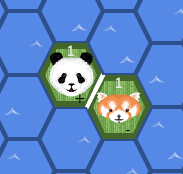
\includegraphics[width=6cm]{pandas_exemple.png}
\end{center}

\newpage

\subsubsection{Bébés pandas}
Les bébés pandas sont votre objectif ! C'est eux que vous devez sauver et qui vous feront gagner la partie. Ils sont toujours sur une case d'eau et ne peuvent pas se déplacer.

\begin{center}
    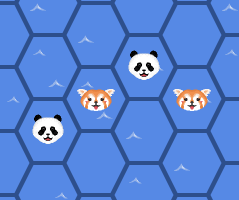
\includegraphics[width=6cm]{bebes_pandas_exemple.png}
\end{center}


\subsection{Déplacements}
Les pandas n'étant pas de grands amateurs des étendues d'eau\footnote{Ils savent bien nager, mais préfèrent éviter de mouiller leur magnifique pelage tout fluffy}, ils préfèrent se déplacer sur des ponts. Ils devront dont construire des ponts en bambou sur la rivière. C'est là qu'ils rencontreront la première grande difficulté : les fonds marins n'ont pas tous la même hauteur et sont très (très) sensibles. Le sable chinois au fond de la rivière de \textit{Hulun} se meut\footnote{Du verbe "mouvoir"} à la moindre perturbation. En plus de construire le pont, marcher dessus changera sa hauteur. Pouvoir passer d'un pont à l'autre pourrait ne plus être garanti à 100\% !

% insérer un screen d'une map avec uniquement des ponts sur l'eau

\section{Règles}
Revoyons ici les règles et modalités plus en détail. Vous êtes lancés sur une rivière constituée de cases hexagonales, deux pandas par joueurs. Les deux pandas sont les parents et se trouvent toujours forcément sur des ponts.

\subsection{Début d'une partie}
Au début, on place deux pandas par race à 4 endroits distincts ($p_1j_1$, $p_2j_1$, $p_1j_2$, $p_2j_2$)\footnote{p = panda, j = joueur}. Les bébés pandas et les ponts sont également placés, dépendamment de la carte chargée.

\subsection{Déroulement d'un tour}
L'ordre des tours est comme suit : panda 1 joueur 1, panda 1 joueur 2, panda 2 joueur 1, panda 2 joueur 2. Pour chaque panda, il est possible d'effectuer trois actions par tour :

\begin{itemize}
    \item Déplacement (ou non)
    \item Pose d'un pont (ou non)
    \item Déplacement (ou non)
\end{itemize}

\subsubsection{Pose d'un pont}
Pour poser un pont, il faut de la place. Vous ne pouvez pas poser un pont sur un bébé panda\footnote{Voir la section Bébés pandas pour comment ramasser un panda}, ni sur un autre pont. Vous ne pouvez pas poser un pont par-dessus un panda, car les pandas sont forcément sur un bout de pont. La valeur d'une case (ou sa hauteur) est uniquement modifiée lorsqu'un panda la \textit{quitte}.

% screen de ponts

\subsubsection{Déplacements}
Vous pouvez toujours vous déplacer d'un côté à l'autre d'un même pont. Ce qui sera la grande difficulté, c'est de passer d'un pont à l'autre. Les ponts ont tous des hauteurs et pour passer d'un pont à l'autre, il faut que la partie du pont sur laquelle vous êtes soit à la même hauteur que la partie du pont où vous voulez aller. Il n'y a pas de nombre de déplacements limités, mais vous ne pouvez pas revenir en arrière lors d'un déplacement atomique\footnote{déplacement atomique = déplacement d'une seule case. Vous pouvez en faire plusieurs, tant que c'est possible. Puis vous vous arrêtez.} !

% screen avec déplacements possibles et impossibles

\subsection{Les bébés pandas}
Les bébés pandas sont ce qui vous rapporte des points\footnote{Voir la partie "Points et Fin de partie"}. Le but est de ramasser tous les bébés. La répartition des bébés par parent panda n'est pas importante. Vous pouvez avoir un seul parent avec tous les bébés, comme les répartir sur les deux parents.

Pour ramasser un bébé panda, il suffit d'être sur une case adjacente. Le ramassage se fera automatiquement.

\subsection{Points et Fin de partie}
Une partie peut s'arrêter pour deux raisons :
\begin{itemize}
    \item une des races de panda a récupéré tous ses bébés
    \item la partie a atteint 200 tours
\end{itemize}

Le calcul se fait comme suit : lorsqu'un bébé panda est ramassé par un parent, il sera porté par ce parent jusqu'à la fin de la partie. Voici ce qu'on fait chaque tour\footnote{Un tour étant à la fin d'un cyce de 4 ponts posés et déplacements faits par les 4 parents pandas sur la map.} pour calculer les points du tour, qui seront additionnés aux points du joueur (classique). Pour chaque parent, on compte son nombre de bébés ramassés. Ce nombre est ensuite multiplié par 5. C'est le nombre de point que rapporte ce parent. Voici un exemple :

Disons qu'un parent panda géant porte un bébé depuis 2 tours et un autre bébé depuis 3 tours. Il aura rapporté au total 3 * 5 + 2 * 5 points depuis le début de la partie. Au tour suivant\footnote{Il faut attendre que les 3 autres aient joué leur tour}, il rapportera 10 points au total\footnote{A condition qu'il ne ramasse pas d'autre bébé pendant ce tour}, car il porte 2 bébés. Ce sont donc 2 * 5 = 10 points.

